%% Week 46 -- Decision trees, bagging and random forests (Chapter 7, Sections
%% 7.1-7.10).  Monday lecture, 2 x 45 min.  Part 1: what a tree is, regression
%% and classification trees, the impurity measures (7.1-7.3).  Part 2: the
%% CART algorithm and its mathematics, done by hand on ten points (7.4).
%% Part 3: the ride data of Table 7.1 -- Gini index and entropy at the root
%% and down the tree, and the same in scikit-learn (7.5).  Part 4: CART from
%% scratch (the listing of 7.6) checked against scikit-learn, regression
%% trees, strengths and weaknesses (7.6-7.7).  Part 5: why averaging helps
%% (Eq. 7.16), bagging and out-of-bag error (7.8-7.9).  Part 6: random
%% forests (7.10), own code and scikit-learn, the moons and the breast-cancer
%% data.  Figures: week46_*.pdf from make_week46_figures.py and the book's
%% chapter-7 figures (impurity_measures, tree_depth_boundary,
%% ensemble_variance).  Companion notebook: week46.ipynb.
%% Book references (book.aux 2026-10-25): Sections 7.1-7.10; Eqs 7.1
%% (tree MSE), 7.2-7.3 (half planes, split criterion), 7.4 (cost complexity),
%% 7.5-7.8 (p_mk, misclassification, Gini, entropy), 7.9-7.10 (CART cost,
%% gain), 7.11-7.12 (CART regression), 7.13 (root Gini of the ride data),
%% 7.14-7.16 (variance of an average), 7.17 (out-of-bag), 7.18 (m = sqrt p);
%% Tables 7.1-7.2; Figs 7.1-7.3.
%% Build:  pdflatex week46slides.tex  (twice)
\documentclass[10pt,aspectratio=169]{beamer}
\usetheme{red_plain}
\usepackage[T1]{fontenc}
\usepackage[utf8]{inputenc}
\usepackage{amsmath,amssymb,bm}
\usepackage{graphicx}
\usepackage{listings}
\usepackage{xcolor}
\usepackage{booktabs}
\usetikzlibrary{trees,positioning}
\graphicspath{{../BookFigures/chapter07_trees_and_ensembles/}{./ch7/}{./}}

%% ---- code listings
\definecolor{codebg}{rgb}{0.97,0.97,0.97}
\lstset{language=Python,basicstyle=\ttfamily\scriptsize,backgroundcolor=\color{codebg},
  keywordstyle=\color{blue!70!black}\bfseries,commentstyle=\color{green!45!black},
  stringstyle=\color{red!60!black},showstringspaces=false,frame=single,
  framerule=0pt,xleftmargin=4pt,xrightmargin=4pt,breaklines=true,columns=fullflexible}

%% ---- the "pause and think" question frames
\newcounter{insight}
\newenvironment{insight}[1][]{%
  \stepcounter{insight}%
  \begin{frame}{Pause and think \arabic{insight}: #1}%
  \setbeamercolor{block title}{bg=structure.fg,fg=white}%
  \setbeamercolor{block body}{bg=structure.fg!8}%
  \small
}{\end{frame}}
\newcommand{\question}[1]{\begin{block}{Question}#1\end{block}}
\newcommand{\answer}[1]{\pause\begin{block}{Answer}#1\end{block}}

\setbeamertemplate{footline}[frame number]
\setbeamerfont{block title}{size=\small}
\setbeamertemplate{blocks}[rounded][shadow=false]
\setbeamercovered{invisible}

\newcommand{\var}{\mathrm{var}}
\newcommand{\cov}{\mathrm{cov}}

\title{Week 46: Decision Trees, Bagging and Random Forests}
\subtitle{A single tree and the mathematics of CART, the Gini index and the
  entropy by hand, a tree from scratch -- then many trees: why averaging
  helps, bagging, and the random forest}
\author{Morten Hjorth-Jensen}
\institute{Department of Physics and Center for Computing in Science Education,\\
  University of Oslo, Norway}
\date{}

\begin{document}

\begin{frame}
\titlepage
\end{frame}

\begin{frame}{Plan for week 46}
\small
\textbf{Monday lecture (2$\times$45 min), the last new topic of the semester:
Chapter 7, Sections 7.1--7.10.}
\begin{enumerate}
  \item \textbf{A single tree}: what it is, regression and classification
        trees, the three impurity measures and why the Gini index and the
        entropy are preferred.
  \item \textbf{The CART algorithm}: the cost it minimises, the gain it
        maximises -- done by hand on ten points, with both criteria.
  \item \textbf{A worked example}: the ride data -- Gini index and entropy at
        the root and down the tree, and the same tree in \texttt{scikit-learn}.
  \item \textbf{A decision tree from scratch}: forty lines of Python,
        checked against \texttt{scikit-learn}; regression trees; strengths and
        weaknesses.
  \item \textbf{Many trees}: why averaging helps (one formula that explains
        the whole chapter), \textbf{bagging} and the out-of-bag error.
  \item \textbf{Random forests}: the one tweak that decorrelates the trees, own
        code and \texttt{scikit-learn}, two data sets.
\end{enumerate}
\textbf{Tuesday (flipped classroom):} about 20 minutes of questions and answers
on today's lecture, then \textbf{Project 3}.\\[2pt]
\textbf{Week 47:} boosting -- AdaBoost, gradient boosting, XGBoost (Sections
7.11--7.15).\\[2pt]
\textbf{A change of plan:} the gated recurrent cells (LSTM and GRU) announced
for today get a separate lecture later; today is trees and forests only.
\end{frame}

\begin{frame}{Reading, and where the code is}
\small
\begin{block}{Chapter 7, Sections 7.1--7.10}
Basics of a tree (7.1), regression trees and pruning (7.2), classification
trees (7.3), the CART algorithm (7.4), the Gini worked example (7.5),
implementing a decision tree (7.6), strengths and weaknesses (7.7), why
averaging helps (7.8), bagging (7.9), random forests (7.10).  Boosting
(7.11--7.15) is next week.
\end{block}
\begin{block}{Other sources}
Hastie, Tibshirani and Friedman, \emph{The Elements of Statistical Learning},
Chapters 9.2, 8.7 and 15; James et al., \emph{An Introduction to Statistical
Learning}, Chapter 8; G\'eron, \emph{Hands-On Machine Learning}, Chapters 6--7;
Raschka et al., Chapter 3 (trees) and 7 (ensembles).
\end{block}
\begin{block}{Code}
Everything shown today, including the from-scratch tree, bagging and forest,
is in \texttt{week46.ipynb} (the functions of
\texttt{make\_week46\_figures.py}).  The book's versions are in
\texttt{BookPrograms/chapter07\_trees\_and\_ensembles/}.
\end{block}
\end{frame}

%=============================================================================
\section{A single tree}
%=============================================================================

\begin{frame}{Every method so far fitted one global function}
\begin{columns}[T]
\begin{column}{0.55\textwidth}
\begin{block}{What we have done}
Linear regression: a hyperplane.  Logistic regression: a sigmoid of a
hyperplane.  Neural networks: compositions of such maps.  In every case
\emph{one} function is adjusted to all the data at once, by a gradient.
\end{block}
\begin{block}{What a tree does instead}
It \textbf{partitions} the feature space into boxes by a sequence of
yes-or-no questions, and fits a \textbf{constant} in each box.  No gradient,
no scaling, no distance.
\end{block}
\end{column}
\begin{column}{0.43\textwidth}
\begin{block}{Why the chapter is interesting}
A tree can be read aloud -- the most interpretable model in the course --
and, on its own, one of the least accurate: \textbf{low bias, very high
variance}.  Fixing that gives bagging, random forests and boosting: on
tabular data, the most accurate methods known.
\end{block}
\end{column}
\end{columns}
\end{frame}

\begin{frame}{The vocabulary (Section 7.1)}
\begin{columns}[T]
\begin{column}{0.5\textwidth}
\begin{itemize}
  \item The \textbf{root node} holds all the observations.
  \item Each \textbf{internal node} tests one feature against a threshold,
        $x_j\le t$, and sends the observation left or right along a
        \textbf{branch}.
  \item Each \textbf{leaf} (terminal node) carries a prediction: a class, or
        a number.
  \item Predicting a new point = walking from the root to a leaf: one
        comparison per level, so the cost is logarithmic in the number of
        leaves.
  \item The \textbf{depth} is the length of the longest walk.
\end{itemize}
\end{column}
\begin{column}{0.48\textwidth}
\centering
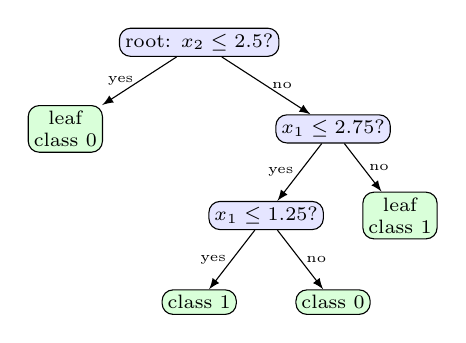
\begin{tikzpicture}[level distance=11mm,
  level 1/.style={sibling distance=34mm},
  level 2/.style={sibling distance=17mm},
  every node/.style={draw,rounded corners,font=\scriptsize,align=center,inner sep=2pt},
  leaf/.style={fill=green!15},
  edge from parent/.style={draw,-latex}]
\node[fill=blue!10]{root: $x_2\le 2.5$?}
  child {node[leaf]{leaf\\class 0}
    edge from parent node[draw=none,left,font=\tiny]{yes}}
  child {node[fill=blue!10]{$x_1\le 2.75$?}
    child {node[fill=blue!10]{$x_1\le 1.25$?}
      child {node[leaf]{class 1} edge from parent node[draw=none,left,font=\tiny]{yes}}
      child {node[leaf]{class 0} edge from parent node[draw=none,right,font=\tiny]{no}}
      edge from parent node[draw=none,left,font=\tiny]{yes}}
    child {node[leaf]{leaf\\class 1} edge from parent node[draw=none,right,font=\tiny]{no}}
    edge from parent node[draw=none,right,font=\tiny]{no}};
\end{tikzpicture}\\[3pt]
\scriptsize The tree we shall grow by hand in Part 2: depth 3, four leaves.
\end{column}
\end{columns}
\end{frame}

\begin{frame}{The geometry: boxes}
\begin{block}{Each test cuts the space with an axis-aligned plane}
$x_j\le t$ is a hyperplane perpendicular to axis $j$.  A tree therefore
partitions the feature space into \textbf{axis-aligned boxes}, one per leaf,
and predicts a constant in each box.
\end{block}
\begin{columns}[T]
\begin{column}{0.49\textwidth}
\begin{block}{The limitation}
Boxes cannot represent a diagonal boundary economically: a tree approximates
$x_1+x_2\le 1$ by a \textbf{staircase}, and needs many leaves to make the
steps small.
\end{block}
\end{column}
\begin{column}{0.49\textwidth}
\begin{block}{The strength}
No notion of distance is needed, so \textbf{no scaling} of the features;
categorical variables and interactions are handled without any special
provision; a monotone transformation of any feature leaves the tree
\emph{unchanged} (which no other method in this course can claim).
\end{block}
\end{column}
\end{columns}
\end{frame}

\begin{frame}{Regression trees (Section 7.2)}
\begin{block}{Two steps}
(1) Split the predictor space into $J$ non-overlapping boxes $R_1,\dots,R_J$.
(2) In box $R_j$ predict the \textbf{mean} $\overline{y}_{R_j}$ of the training
responses that fall in it.
\end{block}
\begin{block}{The goal: boxes that minimise the squared error, Eq.\ (7.1)}
\[
  \sum_{j=1}^{J}\sum_{i\in R_j}\left(y_i-\overline{y}_{R_j}\right)^{2}.
\]
That the best constant in a box is the mean is not an assumption: minimising
$\sum_i(y_i-c)^2$ over $c$ gives $c=\overline{y}$ -- the one-line calculation
that produced the sample mean in Chapter 2.
\end{block}
\begin{block}{The problem}
The number of ways of partitioning the space into $J$ boxes grows
combinatorially.  We cannot search them all, so we proceed \textbf{top-down}
and \textbf{greedily}.
\end{block}
\end{frame}

\begin{frame}{Recursive binary splitting, Eqs.\ (7.2)--(7.3)}
\begin{block}{One step}
Choose a feature $x_j$ and a cutpoint $s$, splitting the current region into
the two half spaces
\[
  R_1(j,s)=\{X\mid x_j<s\},\qquad R_2(j,s)=\{X\mid x_j\ge s\},
\]
so as to minimise
\[
  \sum_{i:\,x_i\in R_1}\left(y_i-\overline{y}_{R_1}\right)^{2}
 +\sum_{i:\,x_i\in R_2}\left(y_i-\overline{y}_{R_2}\right)^{2},
\]
over \emph{all} features $j=1,\dots,p$ and \emph{all} cutpoints $s$.
\end{block}
\begin{columns}[T]
\begin{column}{0.5\textwidth}
\begin{block}{Only $n-1$ cutpoints per feature matter}
The criterion is constant between consecutive sorted values of $x_j$, so
only the midpoints need be tried: one sort per feature, $\mathcal{O}(pn\log n)$
for a split.
\end{block}
\end{column}
\begin{column}{0.48\textwidth}
\begin{block}{Then repeat}
Split one of the two regions just made, then one of the three, \dots\ until
a stopping rule (a minimum number of points per leaf, a maximum depth).
\textbf{Greedy}: the best split \emph{now}, never looking ahead.
\end{block}
\end{column}
\end{columns}
\end{frame}

\begin{insight}[what does a tree do between two data points?]
\question{A regression tree on one feature $x$ has training points at
$x=1,2,3$.  Which thresholds $t$ in ``$x\le t$'' does the algorithm try, and
why not every real number?  And what does the fitted tree predict at $x=10$?}
\answer{Only the midpoints $t=1.5$ and $t=2.5$: every $t\in(1,2)$ puts the
same points left and right, so the criterion~(7.3) does not change; the
midpoint is a convention.  At $x=10$ the point falls into the rightmost leaf
and gets that leaf's mean -- a tree \textbf{cannot extrapolate}; every
prediction is an average of observed targets.  Keep this in mind for the
forests at the end of the lecture: they inherit it.}
\end{insight}

\begin{frame}{Grown to completion, a tree learns nothing: pruning, Eq.\ (7.4)}
\small
\begin{block}{The overfitting signature}
Let the splitting run and every training point ends in its own leaf: zero
training error, and by Chapter 2 no generalisation.  A smaller tree has more
bias but less variance.
\end{block}
\begin{block}{Cost-complexity pruning}
Grow a large tree $T_0$, then for a parameter $\alpha\ge 0$ find the subtree
$T\subset T_0$ minimising
\[
  \sum_{m=1}^{\overline{T}}\;\sum_{i:\,x_i\in R_m}\left(y_i-\overline{y}_{R_m}\right)^{2}
  \;+\;\alpha\,\overline{T},
  \qquad \overline{T}=\text{number of leaves}.
\]
This is training error plus $\alpha$ times a complexity penalty: the
structure of \textbf{Ridge regression}, Eq.\ (3.43), with the number of leaves
in place of $\|\bm{\theta}\|^2$.  Choose $\alpha$ by cross-validation, exactly
as in week 36.  (\texttt{scikit-learn}: \texttt{ccp\_alpha} and
\texttt{cost\_complexity\_pruning\_path}.)
\end{block}
\begin{block}{In practice today}
We shall mostly limit \texttt{max\_depth} and \texttt{min\_samples\_leaf}
instead -- and, from Part 5 on, grow trees deep on purpose and let an
ensemble deal with the variance.
\end{block}
\end{frame}

\begin{frame}{Classification trees (Section 7.3)}
\small
\begin{block}{Two differences from a regression tree}
A leaf predicts the \textbf{majority class} of the training points in it
(and the class proportions give a crude probability).  And the squared error
cannot score a split, so we need a measure of how \emph{impure} a node is.
\end{block}
\begin{block}{The class proportions in a node, Eq.\ (7.5)}
For $K$ classes and the $N_m$ points of region $R_m$,
\[
  p_{mk}=\frac{1}{N_m}\sum_{x_i\in R_m} I(y_i=k),
  \qquad k(m)=\text{the majority class}.
\]
\end{block}
\begin{block}{Three impurity measures, Eqs.\ (7.6)--(7.8)}
\[
  E_m = 1-p_{m,k(m)},\qquad
  G_m = \sum_{k=1}^{K}p_{mk}(1-p_{mk}) = 1-\sum_{k=1}^{K}p_{mk}^{2},\qquad
  S_m = -\sum_{k=1}^{K}p_{mk}\log_2 p_{mk}.
\]
Misclassification rate, \textbf{Gini index}, \textbf{entropy}.  All vanish
for a pure node; all are maximal when the classes are balanced.
\end{block}
\end{frame}

\begin{frame}{Why the Gini index and the entropy, not the error rate}
\begin{columns}[T]
\begin{column}{0.5\textwidth}
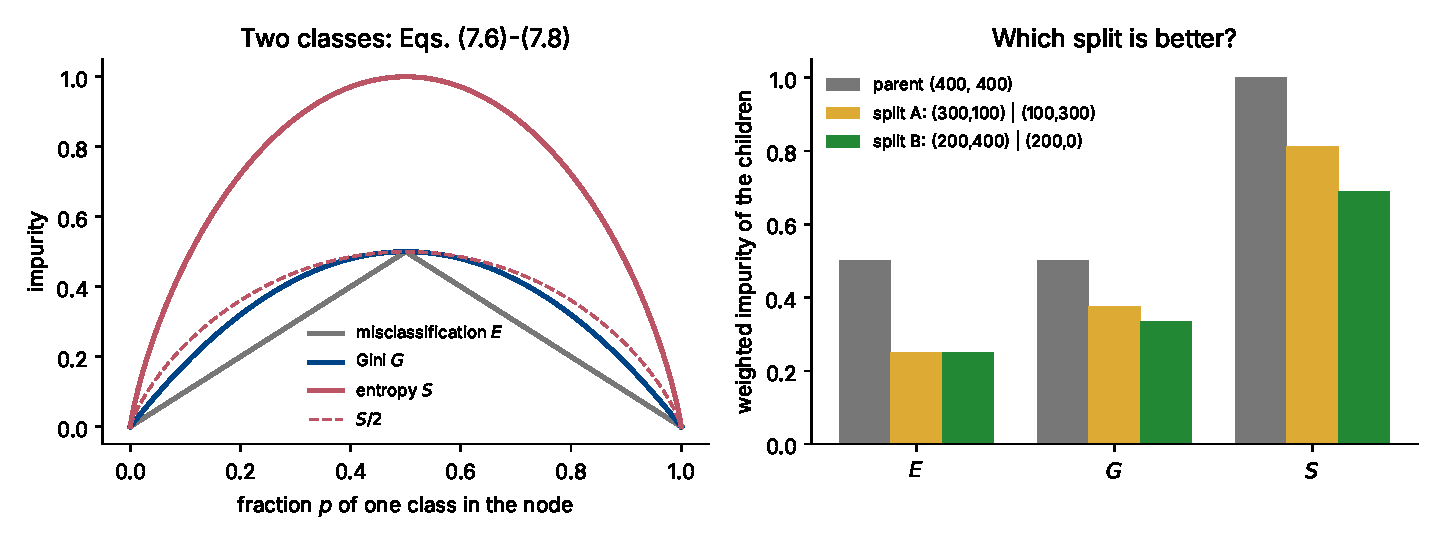
\includegraphics[width=\textwidth]{week46_impurity.pdf}
\end{column}
\begin{column}{0.48\textwidth}
\footnotesize
Two classes, $p$ = fraction of class 1: $E=\min(p,1-p)$ is piecewise linear;
$G=2p(1-p)$ and $S=-p\log_2p-(1-p)\log_2(1-p)$ are \textbf{strictly concave}.

\medskip
A node with $(400,400)$ and two candidate splits:\\
A: $(300,100)\,|\,(100,300)$,\quad B: $(200,400)\,|\,(200,0)$.
\begin{center}\scriptsize
\begin{tabular}{lccc}\toprule
 & $E$ & $G$ & $S$\\\midrule
parent & 0.500 & 0.500 & 1.000\\
after A & 0.250 & 0.375 & 0.811\\
after B & 0.250 & \textbf{0.333} & \textbf{0.689}\\\bottomrule
\end{tabular}
\end{center}
Both splits leave the error rate at $0.25$: $E$ cannot tell them apart.  But
B makes a \textbf{pure} node, and $G$ and $S$ prefer it.  Concavity is the
reason: the weighted average of the children is strictly below the parent
unless the split is trivial, so a split that purifies one branch is rewarded
even when no majority vote changes.  A pure node never needs splitting again.
\end{column}
\end{columns}
\end{frame}

\begin{insight}[the numbers behind the three measures]
\question{A node holds three classes with $12$, $4$ and $4$ points.  Compute
$E$, $G$ and $S$.  Then: what are the largest possible values of $G$ and $S$
for three balanced classes, and for $K$ balanced classes?}
\answer{$p=(0.6,0.2,0.2)$: $E=1-0.6=0.4$;
$G=1-(0.36+0.04+0.04)=0.56$;
$S=-(0.6\log_2 0.6+2\cdot 0.2\log_2 0.2)=0.442+0.929=1.371$ bits.\\[3pt]
Balanced, $p_k=1/K$: $G=1-1/K$ ($=2/3$ for $K=3$) and $S=\log_2 K$
($=1.585$ for $K=3$).  So $G\le 1$ always, while $S$ grows with the number of
classes -- which is why the figure drew $S/2$: for two classes the two
curves are nearly proportional, and in practice they rarely choose different
splits.}
\end{insight}

%=============================================================================
\section{The CART algorithm}
%=============================================================================

\begin{frame}{The CART algorithm (Section 7.4)}
\small
\begin{block}{Classification And Regression Tree -- what \texttt{scikit-learn} implements}
At a node with $m$ points, try every feature $k$ and every threshold $t_k$,
split into left ($x_k\le t_k$) and right, and pick the pair minimising
\[
  C(k,t_k)=\frac{m_{\mathrm{left}}}{m}\,G_{\mathrm{left}}
          +\frac{m_{\mathrm{right}}}{m}\,G_{\mathrm{right}},
  \tag{7.9}
\]
the size-weighted impurity of the two children.  Then do the same in each
child, recursively.
\end{block}
\begin{block}{Equivalently, maximise the impurity decrease -- the \emph{gain}, Eq.\ (7.10)}
\[
  \Delta = G_{\mathrm{parent}}
    -\frac{m_{\mathrm{left}}}{m}G_{\mathrm{left}}
    -\frac{m_{\mathrm{right}}}{m}G_{\mathrm{right}} .
\]
With the entropy in place of $G$, $\Delta$ is the \textbf{information gain},
and choosing splits by it (one branch per value of a categorical feature) is
the \textbf{ID3} algorithm.  Same idea, different impurity, multiway splits.
\end{block}
\begin{block}{Stopping}
A maximum depth, a minimum number of points to split a node or to make a
leaf, a maximum number of leaves, or no split with $\Delta>0$.
\end{block}
\end{frame}

\begin{frame}{CART for regression, Eqs.\ (7.11)--(7.12)}
\begin{block}{Replace the impurity by the mean squared error of the node}
\[
  C(k,t_k)=\frac{m_{\mathrm{left}}}{m}\,\mathrm{MSE}_{\mathrm{left}}
          +\frac{m_{\mathrm{right}}}{m}\,\mathrm{MSE}_{\mathrm{right}},
  \qquad
  \mathrm{MSE}_{\mathrm{node}}=\frac{1}{m_{\mathrm{node}}}\sum_{i\in\mathrm{node}}
  \left(y_i-\overline{y}_{\mathrm{node}}\right)^2 .
\]
This is exactly the split criterion (7.3) divided by $m$, so the two
formulations agree.
\end{block}
\begin{block}{One algorithm, three impurities}
\centering
\begin{tabular}{lll}\toprule
task & node impurity & leaf prediction\\\midrule
regression & $\mathrm{MSE}_{\mathrm{node}}$ (7.12) & mean of $y$\\
classification & Gini $G$ (7.7) or entropy $S$ (7.8) & majority class\\\bottomrule
\end{tabular}
\end{block}
\begin{block}{Everything else is bookkeeping}
Sort each feature once, scan the midpoints, keep the best $(k,t_k)$, recurse.
That is what we shall write in Part 4.
\end{block}
\end{frame}

\begin{frame}{The algorithm as a recipe}
\small
\begin{block}{\textsc{grow}(node with data $(X,y)$, depth $d$)}
\begin{enumerate}
  \item Compute the node's impurity $G_{\mathrm{parent}}$ and its leaf
        prediction (majority class or mean).
  \item If $d=d_{\max}$, or too few points, or the node is pure: return a leaf.
  \item For every feature $k$: sort its values, and for every midpoint $t$
        between consecutive distinct values compute $C(k,t)$ of Eq.\ (7.9)
        and the gain $\Delta=G_{\mathrm{parent}}-C(k,t)$.
  \item Keep the $(k,t)$ with the largest $\Delta$.  If $\Delta\le 0$: return a leaf.
  \item Split the data by $x_k\le t$ and call \textsc{grow} on both halves
        with depth $d+1$.
\end{enumerate}
\end{block}
\begin{block}{Two remarks}
Ties happen (two splits with the same gain); CART breaks them by order or at
random, and that is one reason two implementations can grow different trees
from the same data.  And the search is \textbf{greedy}: the globally best
tree is NP-complete to find; nobody tries.
\end{block}
\end{frame}

\begin{frame}{CART by hand: ten points in the plane}
\begin{columns}[T]
\begin{column}{0.42\textwidth}
\small
\begin{center}
\begin{tabular}{crrc}\toprule
point & $x_1$ & $x_2$ & class\\\midrule
1 & 1.0 & 1.0 & 0\\
2 & 2.0 & 2.0 & 0\\
3 & 3.0 & 2.0 & 0\\
4 & 1.5 & 4.0 & 0\\
5 & 5.0 & 1.0 & 0\\
6 & 4.0 & 4.0 & 1\\
7 & 5.0 & 3.0 & 1\\
8 & 6.0 & 5.0 & 1\\
9 & 1.0 & 5.0 & 1\\
10 & 5.5 & 4.5 & 1\\\bottomrule
\end{tabular}
\end{center}
\end{column}
\begin{column}{0.56\textwidth}
\small
\begin{block}{The root}
Five of each class: $p=(0.5,0.5)$, so $G_{\mathrm{root}}=0.5$ and
$S_{\mathrm{root}}=1$ bit.
\end{block}
\begin{block}{The candidates}
$x_1$ takes the distinct values $1,1.5,2,3,4,5,5.5,6$: seven midpoints
$1.25,1.75,2.5,3.5,4.5,5.25,5.75$.  $x_2$ takes $1,2,3,4,4.5,5$: five
midpoints $1.5,2.5,3.5,4.25,4.75$.  \textbf{Twelve} splits to score.
\end{block}
\begin{block}{One of them, worked out}
$x_2\le 2.5$: left = points $1,2,3,5$, all class 0, $G_{\mathrm{left}}=0$;
right = points $4,6,7,8,9,10$, one class 0 and five class 1,
$G_{\mathrm{right}}=1-(1/6)^2-(5/6)^2=10/36=0.2778$.\\
$C=\tfrac{4}{10}\cdot 0+\tfrac{6}{10}\cdot 0.2778=0.1667$,\quad
$\Delta=0.5-0.1667=\mathbf{0.3333}$.
\end{block}
\end{column}
\end{columns}
\end{frame}

\begin{frame}{All twelve candidates at the root}
\begin{columns}[T]
\begin{column}{0.54\textwidth}
\scriptsize\setlength{\tabcolsep}{3.5pt}
\begin{center}
\begin{tabular}{lcccccc}\toprule
split & $n_{\mathrm{L}}$ & $n_{\mathrm{R}}$ & $C_{\mathrm{Gini}}$ & $\Delta_{\mathrm{Gini}}$ & $C_{\mathrm{ent}}$ & $\Delta_{\mathrm{ent}}$\\\midrule
$x_1\le 1.25$ & 2 & 8 & 0.5000 & 0.0000 & 1.0000 & 0.0000\\
$x_1\le 1.75$ & 3 & 7 & 0.4762 & 0.0238 & 0.9651 & 0.0349\\
$x_1\le 2.5$  & 4 & 6 & 0.4167 & 0.0833 & 0.8755 & 0.1245\\
$x_1\le 3.5$  & 5 & 5 & 0.3200 & 0.1800 & 0.7219 & 0.2781\\
$x_1\le 4.5$  & 6 & 4 & 0.4167 & 0.0833 & 0.8755 & 0.1245\\
$x_1\le 5.25$ & 8 & 2 & 0.3750 & 0.1250 & 0.7635 & 0.2365\\
$x_1\le 5.75$ & 9 & 1 & 0.4444 & 0.0556 & 0.8920 & 0.1080\\\midrule
$x_2\le 1.5$  & 2 & 8 & 0.3750 & 0.1250 & 0.7635 & 0.2365\\
$\mathbf{x_2\le 2.5}$ & 4 & 6 & \textbf{0.1667} & \textbf{0.3333} & \textbf{0.3900} & \textbf{0.6100}\\
$x_2\le 3.5$  & 5 & 5 & 0.3200 & 0.1800 & 0.7219 & 0.2781\\
$x_2\le 4.25$ & 7 & 3 & 0.2857 & 0.2143 & 0.6042 & 0.3958\\
$x_2\le 4.75$ & 8 & 2 & 0.3750 & 0.1250 & 0.7635 & 0.2365\\\bottomrule
\end{tabular}
\end{center}
\end{column}
\begin{column}{0.44\textwidth}
\footnotesize
\begin{block}{Reading the table}
\begin{itemize}
  \item A split that moves one point ($x_1\le 1.25$: points 1 and 9, one of
        each class) gains nothing: the children are as mixed as the parent.
  \item Symmetric splits give symmetric rows ($x_1\le 2.5$ and $x_1\le 4.5$).
  \item $x_2\le 2.5$ wins with both criteria, and by a margin: it creates a
        \textbf{pure} child of four points.
  \item The Gini index and the entropy \emph{rank} the twelve splits
        identically here -- the usual experience.
\end{itemize}
\end{block}
\begin{block}{Then recurse}
The left child is pure: a leaf (class 0).  The right child has six points,
$(1,5)$: scan again, with its own midpoints.
\end{block}
\end{column}
\end{columns}
\end{frame}

\begin{frame}{The gain of every candidate, and the tree that results}
\centering
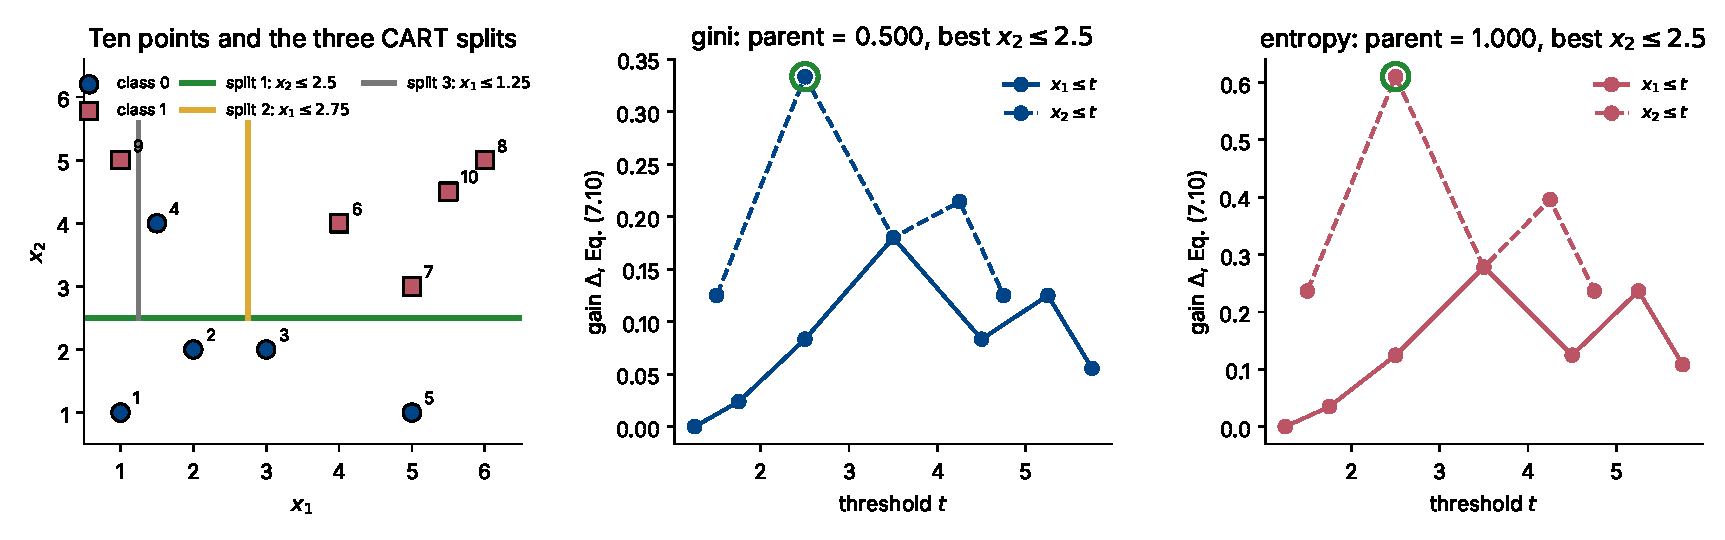
\includegraphics[width=0.98\textwidth]{week46_cart_scan.pdf}\\[2pt]
\small
\begin{columns}[T]
\begin{column}{0.48\textwidth}
\textbf{Split 2}, in the six points above the green line: $x_1\le 2.75$
isolates points 4 and 9 (one of each class) from four class-1 points,
$C=\tfrac{2}{6}\cdot 0.5=0.167$, $\Delta=0.278-0.167=0.111$ -- the best
available.
\end{column}
\begin{column}{0.48\textwidth}
\textbf{Split 3}, in the two remaining points: $x_1\le 1.25$ (or
$x_2\le 4.5$ -- a tie, broken by feature order) separates them.  Depth 3,
four leaves, training error zero.  This is the tree of the vocabulary frame.
\end{column}
\end{columns}
\end{frame}

\begin{insight}[one row of the table by hand]
\question{Verify the row $x_1\le 3.5$ of the table with the Gini index: which
points go left, which right, what are $G_{\mathrm{left}}$,
$G_{\mathrm{right}}$, $C$ and $\Delta$?  Why does this split lose to
$x_2\le 2.5$ although it also balances the classes nicely?}
\answer{Left: points 1, 2, 3, 4 (class 0) and 9 (class 1), proportions
$(4/5,1/5)$, $G_{\mathrm{left}}=1-0.64-0.04=0.32$.  Right: point 5 (class 0)
and 6, 7, 8, 10 (class 1), proportions $(1/5,4/5)$,
$G_{\mathrm{right}}=0.32$.  $C=\tfrac{5}{10}0.32+\tfrac{5}{10}0.32=0.32$,
$\Delta=0.5-0.32=0.18$.\\[3pt]
It leaves one stray point on \emph{each} side, so both children must be
split again; $x_2\le 2.5$ leaves one stray point on one side and none on the
other.  A pure child is worth more to a concave measure than two
nearly-pure ones -- the same lesson as the $(400,400)$ example.}
\end{insight}

%=============================================================================
\section{A worked example: the ride data}
%=============================================================================

\begin{frame}{A worked example with categorical features: the ride data (Table 7.1)}
\begin{columns}[T]
\begin{column}{0.52\textwidth}
\scriptsize\setlength{\tabcolsep}{4pt}
\begin{center}
\begin{tabular}{cllllc}\toprule
Day & Outlook & Temperature & Humidity & Wind & Ride\\\midrule
1 & Sunny & Hot & High & Weak & 0\\
2 & Sunny & Hot & High & Strong & 1\\
3 & Overcast & Hot & High & Weak & 1\\
4 & Rain & Mild & High & Weak & 1\\
5 & Rain & Cool & Normal & Weak & 1\\
6 & Rain & Cool & Normal & Strong & 0\\
7 & Overcast & Cool & Normal & Strong & 1\\
8 & Sunny & Mild & High & Weak & 0\\
9 & Sunny & Cool & Normal & Weak & 1\\
10 & Rain & Mild & Normal & Weak & 1\\
11 & Sunny & Mild & Normal & Strong & 1\\
12 & Overcast & Mild & High & Strong & 1\\
13 & Overcast & Hot & Normal & Weak & 1\\
14 & Rain & Mild & High & Strong & 0\\\bottomrule
\end{tabular}
\end{center}
\end{column}
\begin{column}{0.46\textwidth}
\small
\begin{block}{The question}
From the weather, do we go for a ride?  Four categorical features, a binary
target, fourteen days.
\end{block}
\begin{block}{How a categorical feature is split}
The ID3 way: one child per value (outlook $\to$ sunny, overcast, rain) and
the weighted impurity of Eq.\ (7.9) over all children.  CART (and
\texttt{scikit-learn}) instead makes binary splits on one-hot columns,
``overcast or not?'' -- we shall see both.
\end{block}
\begin{block}{What we compute}
Gini index and entropy at the root, after a split on each feature, then the
same in every impure branch until all leaves are pure.
\end{block}
\end{column}
\end{columns}
\end{frame}

\begin{frame}{The root, Eq.\ (7.13)}
\small
\begin{block}{Ten rides, four non-rides}
\[
  p_{1}=\frac{10}{14},\quad p_{0}=\frac{4}{14}:\qquad
  G_{\mathrm{root}}=1-\left(\tfrac{10}{14}\right)^2-\left(\tfrac{4}{14}\right)^2
  =1-0.5102-0.0816=\mathbf{0.4082},
\]
\[
  S_{\mathrm{root}}=-\tfrac{10}{14}\log_2\tfrac{10}{14}-\tfrac{4}{14}\log_2\tfrac{4}{14}
  =0.3467+0.5164=\mathbf{0.8631}\ \text{bits}.
\]
\end{block}
\begin{block}{Splitting on Outlook: three children}
\centering
\begin{tabular}{lcccc}\toprule
value & days & (no, yes) & $G$ & $S$\\\midrule
Sunny & 1, 2, 8, 9, 11 & (2, 3) & $1-0.16-0.36=0.48$ & 0.971\\
Overcast & 3, 7, 12, 13 & (0, 4) & 0 & 0\\
Rain & 4, 5, 6, 10, 14 & (2, 3) & 0.48 & 0.971\\\bottomrule
\end{tabular}
\[
  C_{\mathrm{Gini}}=\tfrac{5}{14}0.48+\tfrac{4}{14}0+\tfrac{5}{14}0.48=\mathbf{0.3429},
  \qquad
  C_{\mathrm{ent}}=\tfrac{10}{14}0.971=\mathbf{0.6935},
\]
\[
  \text{Gini gain}=0.4082-0.3429=\mathbf{0.0653},\qquad
  \text{information gain}=0.8631-0.6935=\mathbf{0.1696}.
\]
\end{block}
\end{frame}

\begin{frame}{All four features at the root (Table 7.2)}
\begin{columns}[T]
\begin{column}{0.56\textwidth}
\begin{center}
\footnotesize\setlength{\tabcolsep}{2.5pt}
\begin{tabular}{lcccc}\toprule
feature & Gini after & Gini gain & entropy after & info.\ gain\\\midrule
\textbf{Outlook} & \textbf{0.3429} & \textbf{0.0653} & \textbf{0.6935} & \textbf{0.1696}\\
Humidity & 0.3673 & 0.0408 & 0.7885 & 0.0747\\
Temperature & 0.4048 & 0.0034 & 0.8571 & 0.0060\\
Wind & 0.4048 & 0.0034 & 0.8571 & 0.0060\\\bottomrule
\end{tabular}
\end{center}
\footnotesize
Humidity, for the record: High = days 1, 2, 3, 4, 8, 12, 14, counts $(3,4)$,
$G=24/49=0.4898$; Normal = days 5, 6, 7, 9, 10, 11, 13, counts $(1,6)$,
$G=12/49=0.2449$; $C=\tfrac{7}{14}(0.4898+0.2449)=0.3673$.
\end{column}
\begin{column}{0.42\textwidth}
\small
\begin{block}{Both criteria choose Outlook}
And for a visible reason: of its three values, \textbf{overcast is pure} --
all four overcast days are rides -- so that branch is a leaf at once.
Humidity is next best; temperature and wind are nearly useless at the root.
\end{block}
\begin{block}{This is the first step of ID3}
Which attribute best separates the examples?  Select it, make one branch per
value, sort the examples into the branches, repeat in each impure branch.
Greedy, never backtracking.
\end{block}
\end{column}
\end{columns}
\end{frame}

\begin{frame}{Down the tree: the two impure branches}
\footnotesize
\begin{columns}[T]
\begin{column}{0.49\textwidth}
\begin{block}{Rain: days 4, 5, 6, 10, 14, counts $(2,3)$, $G=0.48$}
Wind: Weak = days 4, 5, 10, all rides; Strong = days 6, 14, no rides.  Both
children pure, $C=0$, gain $0.48$ (entropy: gain $0.971$).  Humidity gives
$C=0.4$, Temperature $0.467$.  \textbf{Wind} wins and the branch is finished.
\end{block}
\begin{block}{Sunny: days 1, 2, 8, 9, 11, counts $(2,3)$, $G=0.48$}
Humidity: High = days 1, 2, 8, counts $(2,1)$, $G=0.444$; Normal = days 9,
11, pure.  $C=\tfrac{3}{5}0.444=0.267$.\\
Wind: Weak = days 1, 8, 9, counts $(2,1)$; Strong = days 2, 11, pure.
$C=0.267$ -- \textbf{a tie}.\\
Temperature: Hot $(1,1)$, Mild $(1,1)$, Cool pure: $C=\tfrac{4}{5}0.5=0.4$.\\
Our code takes the first in feature order, Humidity; its High child
$(2,1)$ is then split by Wind: Weak = days 1, 8 (no ride), Strong = day 2
(ride).
\end{block}
\end{column}
\begin{column}{0.49\textwidth}
\begin{block}{The finished tree}
\begin{itemize}
  \item Outlook = Overcast $\to$ ride.
  \item Outlook = Rain $\to$ Wind: Weak $\to$ ride, Strong $\to$ no.
  \item Outlook = Sunny $\to$ Humidity: Normal $\to$ ride; High $\to$
        Wind: Strong $\to$ ride, Weak $\to$ no.
\end{itemize}
Depth 3, seven leaves, every leaf pure, training error zero.
\end{block}
\begin{block}{Gini or entropy?}
The two criteria rank every split the same way at every node here, so they
grow the \textbf{same tree}; only the numbers on the nodes differ.  The tie
on the sunny branch is real for both.
\end{block}
\end{column}
\end{columns}
\end{frame}

\begin{frame}{The ride tree, grown by our code with both criteria}
\centering
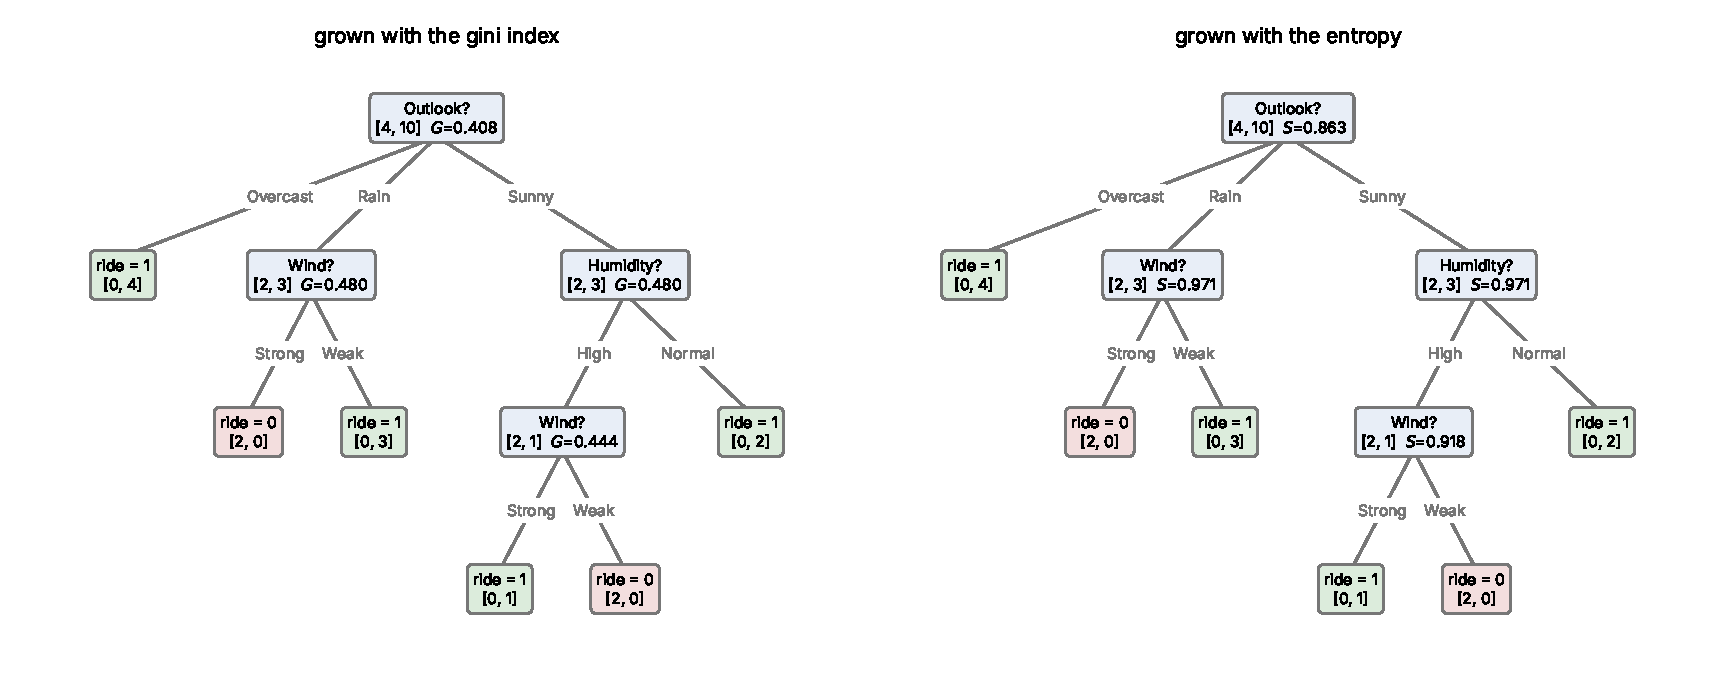
\includegraphics[width=0.92\textwidth]{week46_ride_trees.pdf}\\
\small Node labels: [no rides, rides] and the node impurity.  The code
(\texttt{build\_id3} in the notebook) is fifteen lines: compute the weighted
impurity of Eq.\ (7.9) for every remaining feature, take the smallest, make one
child per value, recurse.
\end{frame}

\begin{frame}[fragile]{The same data in \texttt{scikit-learn}}
\begin{columns}[T]
\begin{column}{0.5\textwidth}
\begin{lstlisting}
from sklearn.preprocessing import OneHotEncoder
from sklearn.tree import (DecisionTreeClassifier,
                          plot_tree, export_text)

X, y, features = ride_data()          # 14 x 4 strings, 0/1
enc = OneHotEncoder(sparse_output=False)
Xoh = enc.fit_transform(X)            # 14 x 10 indicators
names = [n.replace("_", "=")
         for n in enc.get_feature_names_out(features)]

clf = DecisionTreeClassifier(criterion="entropy")
clf.fit(Xoh, y)
print(export_text(clf, feature_names=names))
plot_tree(clf, feature_names=names,
          class_names=["no ride", "ride"], filled=True)
\end{lstlisting}
\end{column}
\begin{column}{0.48\textwidth}
\small
\begin{block}{What is different}
\texttt{scikit-learn} is CART: every split is binary, and a categorical
feature must first be \textbf{one-hot encoded} -- ten indicator columns
``Outlook=Sunny'', ``Wind=Weak'', \dots\ The root asks ``Outlook=Overcast
$\le 0.5$?'', i.e.\ \emph{is it overcast?}, which is our overcast leaf; then
``Humidity=Normal?'', and so on.
\end{block}
\begin{block}{What is the same}
The impurity (\texttt{criterion="gini"} or \texttt{"entropy"}), the greedy
search, pure leaves, training error zero.  Binary splits need more levels:
depth 5 and nine leaves against our depth 3 and seven.
\end{block}
\end{column}
\end{columns}
\end{frame}

\begin{frame}{\texttt{plot\_tree} on the one-hot ride data}
\centering
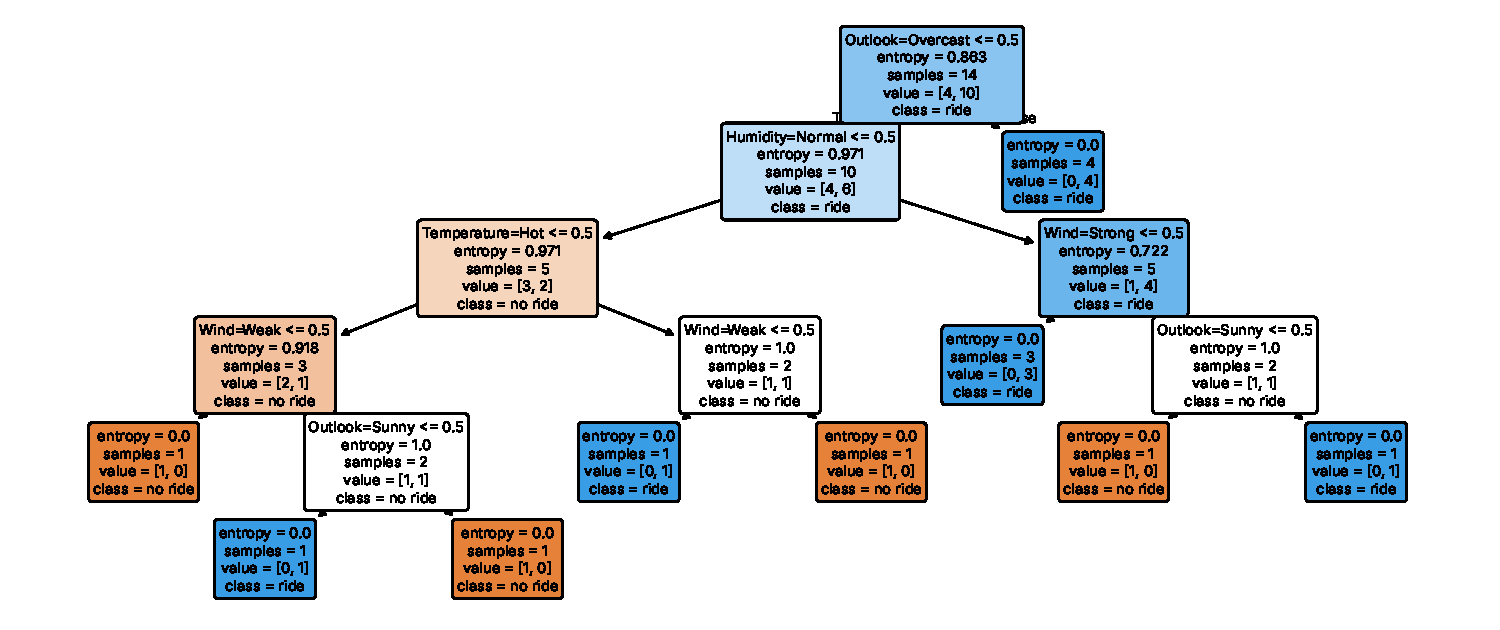
\includegraphics[width=0.9\textwidth]{week46_ride_sklearn.pdf}\\
\small Each box: the test, the node entropy, the number of samples, the
counts [no ride, ride] and the majority class.  Colour saturation is purity.
\end{frame}

%=============================================================================
\section{A decision tree from scratch}
%=============================================================================

\begin{frame}[fragile]{A decision tree from scratch, 1: the impurities and a node (Section 7.6)}
\begin{columns}[T]
\begin{column}{0.5\textwidth}
\begin{lstlisting}
import numpy as np

def gini(y, classes):
    """Eq. (7.7): G = 1 - sum_k p_k^2."""
    p = np.array([np.mean(y == c) for c in classes])
    return 1.0 - np.sum(p**2)

def entropy(y, classes):
    """Eq. (7.8), with 0 log 0 = 0."""
    p = np.array([np.mean(y == c) for c in classes])
    p = p[p > 0]
    return -np.sum(p * np.log2(p))

def mse_impurity(y):
    """Eq. (7.12)."""
    return np.mean((y - y.mean())**2) if len(y) else 0.0
\end{lstlisting}
\end{column}
\begin{column}{0.48\textwidth}
\begin{lstlisting}
class Node:
    __slots__ = ("feature", "threshold",
                 "left", "right", "value", "n")

    def __init__(self, value=None, n=0):
        self.feature = self.threshold = None
        self.left = self.right = None
        self.value, self.n = value, n
\end{lstlisting}
\small
\begin{block}{The data structure}
A node is either a \textbf{test} (\texttt{feature}, \texttt{threshold}, two
children) or a \textbf{leaf} (\texttt{feature is None}); every node stores
its prediction \texttt{value}, so any node can be a leaf if we stop there.
\end{block}
\end{column}
\end{columns}
\end{frame}

\begin{frame}[fragile]{A decision tree from scratch, 2: the class}
\begin{lstlisting}
class DecisionTree:
    """CART for regression and classification.
    task: "classification" or "regression";  criterion: "gini" or "entropy";
    max_features: if set, only a random subset of features is tried at each split
                  -- this is what turns bagging into a random forest (Part 6)."""

    def __init__(self, task="classification", criterion="gini", max_depth=None,
                 min_samples_split=2, min_samples_leaf=1, max_features=None, rng=None):
        self.task, self.criterion = task, criterion
        self.max_depth = np.inf if max_depth is None else max_depth
        self.min_samples_split, self.min_samples_leaf = min_samples_split, min_samples_leaf
        self.max_features = max_features
        self.rng = np.random.default_rng() if rng is None else rng

    def _impurity(self, y):
        if self.task == "regression":
            return mse_impurity(y)
        return gini(y, self.classes_) if self.criterion == "gini" else entropy(y, self.classes_)

    def _leaf_value(self, y):
        if self.task == "regression":
            return y.mean()                                   # the optimal constant
        counts = [np.sum(y == c) for c in self.classes_]
        return self.classes_[int(np.argmax(counts))]          # majority vote
\end{lstlisting}
\end{frame}

\begin{frame}[fragile]{A decision tree from scratch, 3: the best split -- Eqs.\ (7.9)--(7.10)}
\begin{lstlisting}
    def _best_split(self, X, y):
        n, p = X.shape
        features = np.arange(p)
        if self.max_features is not None and self.max_features < p:
            features = self.rng.choice(p, self.max_features, replace=False)   # random forest
        parent = self._impurity(y)
        best_gain, best_j, best_t = 0.0, None, None
        for j in features:
            xs = X[:, j]
            uniq = np.unique(xs)                              # sorted distinct values
            if len(uniq) < 2:
                continue
            for t in (uniq[:-1] + uniq[1:]) / 2.0:            # candidate midpoints
                mask = xs <= t
                nl, nr = mask.sum(), n - mask.sum()
                if nl < self.min_samples_leaf or nr < self.min_samples_leaf:
                    continue
                child = (nl / n) * self._impurity(y[mask]) + (nr / n) * self._impurity(y[~mask])
                gain = parent - child                         # Eq. (7.10)
                if gain > best_gain + 1e-12:                  # first maximum wins a tie
                    best_gain, best_j, best_t = gain, j, t
        return best_gain, best_j, best_t
\end{lstlisting}
\small This is the recipe frame, line for line: the double loop over
features and midpoints, $C(k,t)$ as \texttt{child}, the gain, the argmax.
\end{frame}

\begin{frame}[fragile]{A decision tree from scratch, 4: grow, fit, predict}
\begin{columns}[T]
\begin{column}{0.56\textwidth}
\begin{lstlisting}
    def _build(self, X, y, depth):
        node = Node(self._leaf_value(y), len(y))
        if (depth >= self.max_depth or len(y) < self.min_samples_split
                or len(np.unique(y)) == 1):           # stopping rules
            return node
        gain, j, t = self._best_split(X, y)
        if j is None or gain <= 0:
            return node
        mask = X[:, j] <= t
        node.feature, node.threshold = j, t
        node.left = self._build(X[mask], y[mask], depth + 1)
        node.right = self._build(X[~mask], y[~mask], depth + 1)
        return node

    def fit(self, X, y):
        X, y = np.asarray(X, dtype=float), np.asarray(y)
        if self.task == "classification":
            self.classes_ = np.unique(y)
        self.root_ = self._build(X, y, 0)
        return self
\end{lstlisting}
\end{column}
\begin{column}{0.42\textwidth}
\begin{lstlisting}
    def predict(self, X):
        X = np.asarray(X, dtype=float)
        out = []
        for x in X:
            node = self.root_
            while node.feature is not None:   # walk to a leaf
                node = (node.left if x[node.feature] <= node.threshold
                        else node.right)
            out.append(node.value)
        return np.array(out)
\end{lstlisting}
\small
\begin{block}{That is all}
Recursion does the bookkeeping; the whole class is under sixty lines and
handles regression, two impurities, depth and leaf-size limits, and the
random feature subset we need in Part 6.
\end{block}
\end{column}
\end{columns}
\end{frame}

\begin{frame}{Checking it against \texttt{scikit-learn}: the moons}
\begin{columns}[T]
\begin{column}{0.52\textwidth}
\small
Moons data (week 39), $n=400$, noise $0.3$, 300 training and 100 test
points, Gini index, both implementations:
\begin{center}
\setlength{\tabcolsep}{4pt}
\begin{tabular}{lcccc}\toprule
 & \multicolumn{2}{c}{ours} & \multicolumn{2}{c}{\texttt{scikit-learn}}\\
depth & train & test & train & test\\\midrule
1 & 0.8267 & 0.7800 & 0.8267 & 0.7800\\
3 & 0.9000 & 0.8600 & 0.9000 & 0.8600\\
5 & 0.9633 & 0.8600 & 0.9633 & 0.8600\\
unlimited & 1.0000 & 0.8600 & 1.0000 & 0.8400\\\bottomrule
\end{tabular}
\end{center}
Leaves: 2, 7, 18 and 33 in both.  The whole unlimited tree takes $0.1$ s in
pure Python.
\end{column}
\begin{column}{0.46\textwidth}
\begin{block}{Identical where it should be}
Same accuracies, same number of leaves at every depth.  At unlimited depth
the test accuracies differ by two points out of a hundred: \textbf{ties}
between equally good splits, broken differently.
\end{block}
\begin{block}{The last row is the lesson}
The fully grown tree fits the training data perfectly and generalises
\emph{no better} than depth 3 -- here slightly worse for
\texttt{scikit-learn}.  The variance term of the bias-variance
decomposition, Eq.\ (2.52), growing without limit.  Everything from Part 5
on is a way of controlling it.
\end{block}
\end{column}
\end{columns}
\end{frame}

\begin{frame}{What the depth does to the boundary (book Figure 7.2)}
\centering
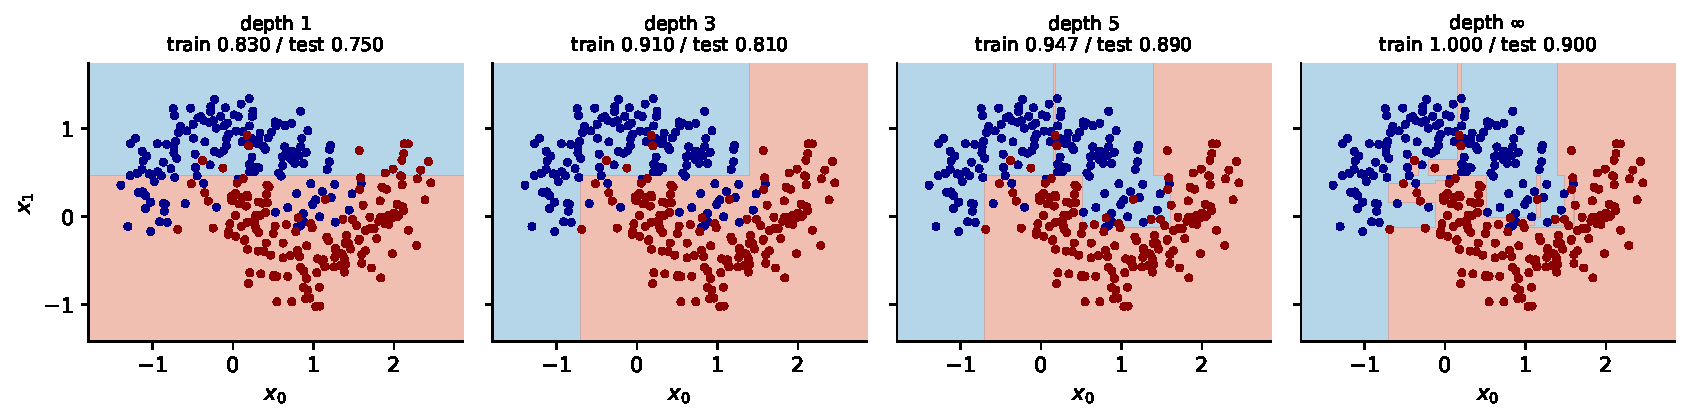
\includegraphics[width=0.9\textwidth]{tree_depth_boundary.pdf}\\
\small At depth one a single threshold; at depth three the right gross
shape; at depth five close to the truth; grown without limit, narrow
rectangular islands around individual training points.  Every boundary is a
staircase of axis-aligned steps.
\end{frame}

\begin{frame}{Regression trees are staircases, and deeper is not better}
\centering
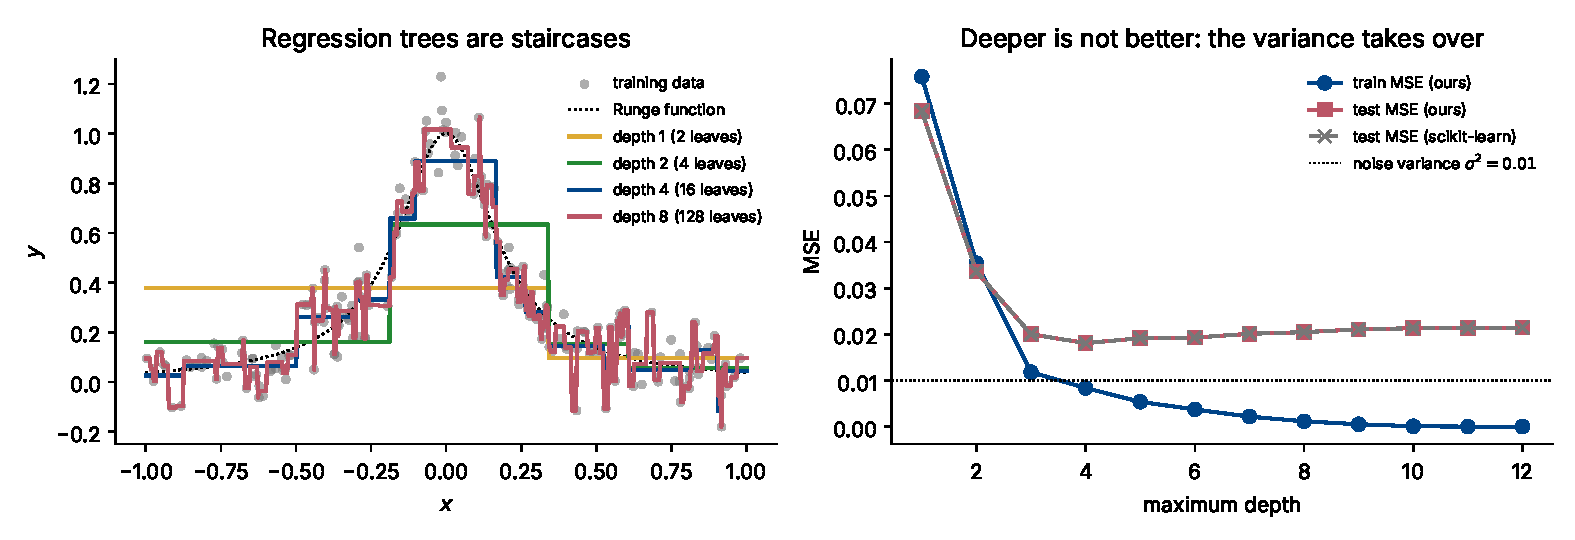
\includegraphics[width=0.98\textwidth]{week46_regression_tree.pdf}\\
\small
The Runge function with noise $\sigma=0.1$, 200 training and 200 test points,
our \texttt{DecisionTree("regression")}.  A depth-$d$ tree has at most $2^d$
leaves, each a constant.  Train MSE falls to zero; test MSE is smallest at
depth 4 ($0.0181$), then rises to $0.0214$ at full depth -- and never reaches
the noise floor $0.01$ that a degree-10 polynomial ($0.0133$) gets close to.
A tree is the wrong tool for one smooth feature; \texttt{scikit-learn} gives
the same test numbers to four digits.
\end{frame}

\begin{frame}[fragile]{Trees in \texttt{scikit-learn}: what you will actually call}
\begin{columns}[T]
\begin{column}{0.52\textwidth}
\begin{lstlisting}[basicstyle=\ttfamily\tiny]
from sklearn.tree import (DecisionTreeClassifier,
                          DecisionTreeRegressor, plot_tree)
from sklearn.model_selection import (train_test_split,
                                     GridSearchCV)

clf = DecisionTreeClassifier(criterion="gini",   # or "entropy"
                             max_depth=5,
                             min_samples_leaf=5,
                             random_state=0)
clf.fit(X_train, y_train)
print(clf.score(X_test, y_test))
print(clf.get_depth(), clf.get_n_leaves())
print(clf.feature_importances_)       # Gini decrease per feature
plot_tree(clf, filled=True, feature_names=names)

# choose the depth / leaf size / pruning by cross-validation
grid = GridSearchCV(DecisionTreeClassifier(random_state=0),
                    {"max_depth": [2, 3, 4, 6, 8, None],
                     "min_samples_leaf": [1, 5, 10],
                     "ccp_alpha": [0.0, 1e-3, 1e-2]},
                    cv=5).fit(X_train, y_train)
print(grid.best_params_, grid.best_score_)

reg = DecisionTreeRegressor(max_depth=4).fit(X_train, y_train)
\end{lstlisting}
\end{column}
\begin{column}{0.46\textwidth}
\footnotesize
\begin{block}{The knobs, and what they are in our code}
\texttt{criterion} = \texttt{gini}/\texttt{entropy} (\texttt{squared\_error}
for the regressor); \texttt{max\_depth}, \texttt{min\_samples\_split},
\texttt{min\_samples\_leaf} = the three stopping rules of \texttt{\_build};
\texttt{max\_features} = the random subset in \texttt{\_best\_split};
\texttt{ccp\_alpha} = the $\alpha$ of Eq.\ (7.4).
\end{block}
\begin{block}{Two habits}
No scaling pipeline is needed (it would change nothing).  Cross-validate the
depth or $\alpha$ exactly as you cross-validated $\lambda$ in Project 1 and
the learning rate in Project 2 -- the week-44 machinery applies unchanged.
\end{block}
\end{column}
\end{columns}
\end{frame}

\begin{frame}{Strengths and weaknesses of a single tree (Section 7.7)}
\begin{columns}[T]
\begin{column}{0.49\textwidth}
\begin{block}{In favour}
\begin{itemize}
  \item Simple to understand, to interpret, to draw: a \textbf{white box} --
        any prediction is explained by its sequence of tests.
  \item Little data preparation: no scaling or centring; invariant under
        monotone transformations of the features.
  \item Prediction costs $\mathcal{O}(\text{depth})$.
  \item Numerical and categorical features, multiple outputs, missing values
        (with some care).
\end{itemize}
\end{block}
\end{column}
\begin{column}{0.49\textwidth}
\begin{block}{Against}
\begin{itemize}
  \item \textbf{Overfits} readily: depth limits, leaf sizes or pruning are
        mandatory.
  \item \textbf{Unstable}: a small change in the data can give a completely
        different tree -- the high variance we just measured.
  \item Greedy: no guarantee of the best tree (NP-complete anyway).
  \item Staircases for diagonal boundaries; biased towards features with many
        split points and towards the majority class.
\end{itemize}
\end{block}
\end{column}
\end{columns}
\begin{block}{The crucial defect is the opportunity}
A low-bias, high-variance, \emph{unstable} predictor is exactly what averaging
helps most.  The rest of the lecture follows from that one observation.
\end{block}
\end{frame}

\begin{insight}[scaling, logarithms and trees]
\question{You standardise every feature (subtract the mean, divide by the
standard deviation) before fitting (a) a decision tree, (b) Ridge
regression, (c) a neural network trained with SGD.  Which fits change?  And
if instead you replace a feature $x_j$ by $\log x_j$ ($x_j>0$)?}
\answer{(a) \textbf{Nothing} changes, in either case: a test $x_j\le t$
becomes $(x_j-\mu)/\sigma\le(t-\mu)/\sigma$, or $\log x_j\le\log t$ -- the
same points go left and right at every candidate split, so the same tree is
grown with the same gains.  Any strictly monotone map of a feature leaves a
tree invariant.\\
(b) Ridge changes under both: the penalty $\lambda\|\bm{\theta}\|^2$ weighs
coefficients whose meaning depends on the units, and $\log x_j$ is a
different model.  (c) The network's fit changes too (conditioning of the
optimisation, and $\log x_j$ is a different input), which is why weeks 37--41
insisted on scaling.  Trees are the one method in the course for which the
advice ``scale your data'' is void.}
\end{insight}

%=============================================================================
\section{Many trees: why averaging helps, and bagging}
%=============================================================================

\begin{frame}{Why averaging helps (Section 7.8): independent predictors, Eq.\ (7.14)}
\begin{block}{Average $B$ predictors}
$\hat f_1,\dots,\hat f_B$, each unbiased for the target with variance
$\sigma^2$, and $\bar f=\frac1B\sum_b\hat f_b$.  If they are
\textbf{independent},
\[
  \mathbb{E}[\bar f]=\mathbb{E}[\hat f_b],\qquad
  \var(\bar f)=\frac{\sigma^2}{B}.
\]
\end{block}
\begin{block}{Read against the bias-variance decomposition, Eq.\ (2.52)}
The bias is untouched; the variance falls as $1/B$.  Averaging attacks the
\textbf{variance term only}.  That is why it is the right treatment for
\emph{deep} trees (bias already small, variance huge) and the wrong one for a
model that is too rigid -- averaging a hundred straight lines gives a
straight line.
\end{block}
\begin{block}{The catch}
Predictors fitted to the same data set are \emph{not} independent.
\end{block}
\end{frame}

\begin{frame}{The central formula of the chapter, Eqs.\ (7.15)--(7.16)}
\begin{block}{Pairwise correlation $\rho$}
\[
  \var(\bar f)=\frac{1}{B^2}\Big[\sum_b\var(\hat f_b)+\sum_{b\ne b'}\cov(\hat f_b,\hat f_{b'})\Big]
  =\frac{1}{B^2}\Big[B\sigma^2+B(B-1)\rho\sigma^2\Big],
\]
which simplifies to
\[
  \boxed{\;\var(\bar f)=\rho\,\sigma^2+\frac{1-\rho}{B}\,\sigma^2 .\;}
\]
\end{block}
\begin{columns}[T]
\begin{column}{0.49\textwidth}
\begin{block}{Read it carefully}
The second term vanishes as $B\to\infty$: more predictors always help, with
diminishing returns.  The first term does \textbf{not depend on $B$}: however
many trees we average, the variance cannot fall below $\rho\sigma^2$.
\end{block}
\end{column}
\begin{column}{0.49\textwidth}
\begin{block}{The design specification}
Make $\sigma^2$ small (accurate members), $B$ large (many members), and --
easy to overlook -- $\rho$ small (\textbf{diverse} members).  Bagging
attacks $\sigma^2/B$; random forests exist because bagging leaves $\rho$ too
large; boosting (next week) attacks the bias instead.
\end{block}
\end{column}
\end{columns}
\end{frame}

\begin{frame}{Eq.\ (7.16) measured on bagged trees, and Condorcet's jury}
\centering
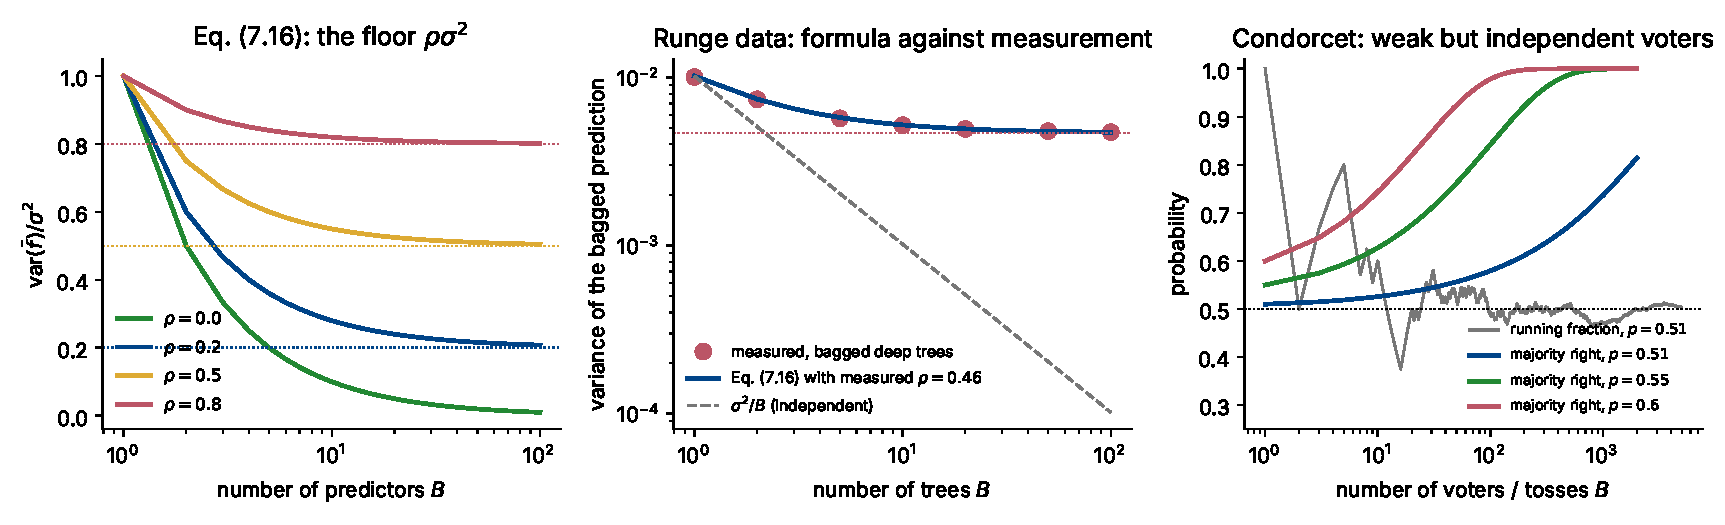
\includegraphics[width=0.98\textwidth]{week46_variance.pdf}\\
\small
\textbf{Left}: the formula; dotted lines are the floors $\rho\sigma^2$.
\textbf{Middle}: 200 independent training sets of the noisy Runge function,
100 deep trees on bootstrap samples of each; measured $\sigma^2=0.0102$ for
one tree, measured $\rho=0.46$ between two trees of the same ensemble, and
the variance of the average of $B$ of them -- the formula with these two
numbers, no fitting.  Averaging 100 trees removes half the variance and then
stops.  \textbf{Right}: $B$ independent voters each right with probability
$p$: a majority of 1001 voters with $p=0.55$ is right with probability
$0.999$; with $p=0.51$, $0.737$.  Weak but independent voters combine into a
strong one -- the italics are the assumption reality violates.
\end{frame}

\begin{frame}{Bagging (Section 7.9): bootstrap aggregation}
\begin{block}{The recipe}
We cannot draw $B$ independent training sets -- we have one.  So we
manufacture them by the \textbf{bootstrap} of week 36: draw $n$ observations
\emph{with replacement}, fit a tree, repeat $B$ times, and \textbf{average}
the predictions (regression) or take a \textbf{majority vote}
(classification).
\end{block}
\begin{columns}[T]
\begin{column}{0.49\textwidth}
\begin{block}{Grow the trees deep and do not prune}
Deliberate: deep trees have low bias and high variance; averaging removes
variance and leaves bias.  We want the members as unbiased as possible and
let the ensemble handle the rest.
\end{block}
\end{column}
\begin{column}{0.49\textwidth}
\begin{block}{What it costs}
$B$ fits instead of one (embarrassingly parallel), $B$ trees to store and
walk at prediction time, and the readable tree is gone: a hundred trees
cannot be drawn as one.
\end{block}
\end{column}
\end{columns}
\end{frame}

\begin{frame}{A free validation set: the out-of-bag error, Eq.\ (7.17)}
\begin{block}{A third of the data misses each tree}
The probability that a given observation is \emph{not} drawn in one
bootstrap sample of size $n$ is
\[
  \Big(1-\frac1n\Big)^{n}\;\longrightarrow\;e^{-1}\approx 0.368
  \qquad(n\to\infty).
\]
Measured in our implementation: $0.3693$ against $0.3679$.
\end{block}
\begin{block}{Out-of-bag prediction}
For each observation, average (or let vote) only the trees that did
\textbf{not} see it -- about $0.37B$ of them.  The resulting error is an
almost unbiased estimate of the test error, with no separate split and no
cross-validation loop.  In \texttt{scikit-learn}: \texttt{oob\_score=True}.
\end{block}
\begin{block}{What survives of interpretability}
\textbf{Variable importance}: the total decrease of impurity (MSE or Gini)
due to splits on each feature, summed over all trees and normalised.  A
summary, not an explanation -- and known to favour features with many
distinct values.
\end{block}
\end{frame}

\begin{frame}[fragile]{Bagging from scratch, 1: fit and predict}
\begin{lstlisting}[basicstyle=\ttfamily\tiny]
class BaggingClassifier:
    """Bootstrap aggregation of unpruned trees, with out-of-bag scoring."""

    def __init__(self, n_estimators=100, max_depth=None, max_features=None, rng=None):
        self.n_estimators, self.max_depth = n_estimators, max_depth
        self.max_features = max_features
        self.rng = np.random.default_rng(0) if rng is None else rng

    def fit(self, X, y):
        X, y = np.asarray(X, dtype=float), np.asarray(y)
        n = len(y)
        self.classes_ = np.unique(y)
        self.trees_, self.oob_ = [], []
        for _ in range(self.n_estimators):
            idx = self.rng.integers(0, n, n)                 # bootstrap resample, with replacement
            self.oob_.append(np.setdiff1d(np.arange(n), idx))  # points this tree never sees
            tree = DecisionTree("classification", "gini", max_depth=self.max_depth,
                                max_features=self.max_features, rng=self.rng)
            self.trees_.append(tree.fit(X[idx], y[idx]))
        return self

    def predict(self, X):
        X = np.asarray(X, dtype=float)
        votes = np.stack([t.predict(X) for t in self.trees_])  # (B, n_points)
        out = np.empty(X.shape[0], dtype=self.classes_.dtype)
        for i in range(X.shape[0]):                          # majority vote
            counts = [np.sum(votes[:, i] == c) for c in self.classes_]
            out[i] = self.classes_[int(np.argmax(counts))]
        return out
\end{lstlisting}
\end{frame}

\begin{frame}[fragile]{Bagging from scratch, 2: the out-of-bag score}
\begin{columns}[T]
\begin{column}{0.56\textwidth}
\begin{lstlisting}
    def oob_score(self, X, y):
        """Eq. (7.17): each point is scored only by
        the trees that never saw it."""
        X, y = np.asarray(X, dtype=float), np.asarray(y)
        tally = np.zeros((len(y), len(self.classes_)))
        for tree, oob in zip(self.trees_, self.oob_):
            if len(oob) == 0:
                continue
            pred = tree.predict(X[oob])
            for k, c in enumerate(self.classes_):
                tally[oob[pred == c], k] += 1
        seen = tally.sum(axis=1) > 0
        vote = self.classes_[np.argmax(tally[seen], axis=1)]
        return np.mean(vote == y[seen])
\end{lstlisting}
\end{column}
\begin{column}{0.42\textwidth}
\small
\begin{block}{Reading it}
\texttt{tally[i, k]} counts how many of the trees that did not train on
point $i$ voted for class $k$.  Each point gets about $0.37B$ votes; with
$B=100$ every point is \texttt{seen} in practice.  The majority of those
votes is the out-of-bag prediction.
\end{block}
\begin{block}{Why it is honest}
No tree that votes on point $i$ has ever seen $y_i$: exactly the situation
of a test point, obtained from the training set alone.
\end{block}
\end{column}
\end{columns}
\end{frame}

\begin{frame}[fragile]{Bagging in \texttt{scikit-learn}}
\begin{columns}[T]
\begin{column}{0.54\textwidth}
\begin{lstlisting}
from sklearn.ensemble import (BaggingClassifier,
                              BaggingRegressor)
from sklearn.tree import DecisionTreeClassifier

bag = BaggingClassifier(
        estimator=DecisionTreeClassifier(),  # deep, unpruned
        n_estimators=100,
        max_samples=1.0,       # bootstrap sample of size n
        bootstrap=True,        # with replacement
        oob_score=True,        # Eq. (7.17)
        n_jobs=-1,             # trees are independent: parallel
        random_state=0)
bag.fit(X_train, y_train)
print(bag.oob_score_, bag.score(X_test, y_test))
print(len(bag.estimators_))   # the 100 trees
print(bag.predict_proba(X_test)[:3])   # vote fractions

# regression: averages instead of votes
breg = BaggingRegressor(n_estimators=200, oob_score=True)
\end{lstlisting}
\end{column}
\begin{column}{0.44\textwidth}
\small
\begin{block}{Line by line}
\texttt{estimator} is the base learner -- any estimator works, trees are
the standard choice; \texttt{max\_samples=1.0} and \texttt{bootstrap=True}
give the bootstrap of Eq.\ (7.17); \texttt{oob\_score=True} makes the free
validation estimate available as \texttt{oob\_score\_};
\texttt{predict\_proba} returns the fraction of trees voting for each class.
\end{block}
\begin{block}{The one parameter}
$B$ = \texttt{n\_estimators}.  By Eq.\ (7.16) more trees never hurt, they
only stop helping; choose by budget, and watch \texttt{oob\_score\_}
flatten.
\end{block}
\end{column}
\end{columns}
\end{frame}

%=============================================================================
\section{Random forests}
%=============================================================================

\begin{frame}{Random forests (Section 7.10): one tweak that decorrelates the trees}
\begin{block}{As bagging, plus}
Each time a split is considered, only a \textbf{random sample of $m$ of the $p$
features} is offered as candidates, and the split must use one of them.  A
fresh sample at every split.  Typically
\[
  m\approx\sqrt{p}\quad\text{(classification)},\qquad m\approx p/3\quad\text{(regression)}.
  \tag{7.18}
\]
At each split the algorithm is \emph{not allowed} to look at most of the
features.
\end{block}
\begin{block}{In our code it is one line}
The \texttt{max\_features} branch of \texttt{\_best\_split}:
\texttt{features = rng.choice(p, max\_features, replace=False)}.
\end{block}
\end{frame}

\begin{frame}{Why this clever restriction works}
\begin{columns}[T]
\begin{column}{0.49\textwidth}
\begin{block}{The problem with bagging}
Suppose one feature is very strong and several others moderately strong.
Almost every bagged tree puts the strong feature at its root; the trees look
alike and their predictions are \textbf{highly correlated}.  By Eq.\ (7.16)
the floor $\rho\sigma^2$ is high and more trees do not help.
\end{block}
\begin{block}{The cure}
With $m$ of $p$ features per split, the strong feature is unavailable in a
fraction $1-m/p$ of the splits; other features get their turn, and the trees
\emph{genuinely differ}: $\rho$ falls.
\end{block}
\end{column}
\begin{column}{0.49\textwidth}
\begin{block}{The price}
Each tree is worse than it could be: $\sigma^2$ rises.  Random forests work
because, for deep trees, the fall in $\rho$ outweighs the rise in
$\sigma^2$ -- and $m$ is the hyperparameter trading them off.
\end{block}
\begin{block}{The two limits}
$m=p$ is bagging exactly.  $m=1$ gives maximally decorrelated but very weak
trees (the split \emph{feature} is random, only the threshold is chosen).
Eq.\ (7.18) is a rule of thumb; $m$ deserves cross-validation like any other
hyperparameter.
\end{block}
\end{column}
\end{columns}
\end{frame}

\begin{frame}[fragile]{A random forest from scratch: a subclass}
\begin{columns}[T]
\begin{column}{0.5\textwidth}
\begin{lstlisting}
class RandomForestClassifier(BaggingClassifier):
    """Bagging plus a random subset of
    m features at every split."""

    def __init__(self, n_estimators=100, max_depth=None,
                 max_features="sqrt", rng=None):
        super().__init__(n_estimators, max_depth, None, rng)
        self._mf = max_features

    def fit(self, X, y):
        p = np.asarray(X).shape[1]
        self.max_features = (int(np.sqrt(p))
                             if self._mf == "sqrt" else self._mf)
        return super().fit(X, y)          # Eq. (7.18)
\end{lstlisting}
\end{column}
\begin{column}{0.48\textwidth}
\small
\begin{block}{Where the randomness enters}
Twice: the bootstrap sample of each tree (inherited from
\texttt{BaggingClassifier.fit}), and the feature subset drawn
\emph{inside every call} of \texttt{\_best\_split}, because
\texttt{max\_features} is passed down to each \texttt{DecisionTree}.
\end{block}
\begin{block}{A detail}
On the moons $p=2$, so $m=\lfloor\sqrt2\rfloor=1$: every split picks its
feature at random.  On the cancer data below, $p=30$ and $m=5$.
\end{block}
\end{column}
\end{columns}
\end{frame}

\begin{frame}{Single tree, bagging, forest on the moons}
\begin{columns}[T]
\begin{column}{0.5\textwidth}
\small
$n=500$, noise $0.3$, 375 training and 125 test points, $B=100$ deep trees:
\begin{center}
\setlength{\tabcolsep}{4pt}
\begin{tabular}{lcc}\toprule
 & test accuracy & out-of-bag\\\midrule
single tree (ours) & 0.824 & --\\
single tree (\texttt{sklearn}) & 0.824 & --\\
bagging (ours) & 0.896 & 0.907\\
bagging (\texttt{sklearn}) & 0.872 & 0.923\\
forest (ours) & 0.880 & 0.909\\
forest (\texttt{sklearn}) & 0.880 & 0.915\\\bottomrule
\end{tabular}
\end{center}
Out-of-bag fraction measured: $0.3693$ ($1/e=0.3679$).
\end{column}
\begin{column}{0.48\textwidth}
\begin{block}{What is significant and what is not}
Both ensembles beat the single tree by five to seven points.  Between the
four ensemble numbers the differences are \emph{not} significant: for an
accuracy near $0.9$ on 125 points the standard error, Eq.\ (2.24), is
$\sqrt{0.9\cdot 0.1/125}\approx 0.027$.
\end{block}
\begin{block}{Trust the out-of-bag numbers more}
They use all 375 training points.  They agree: around $0.91$--$0.92$ for
every ensemble, against $0.82$ for one tree.
\end{block}
\end{column}
\end{columns}
\end{frame}

\begin{frame}{What the ensembles do to the boundary}
\centering
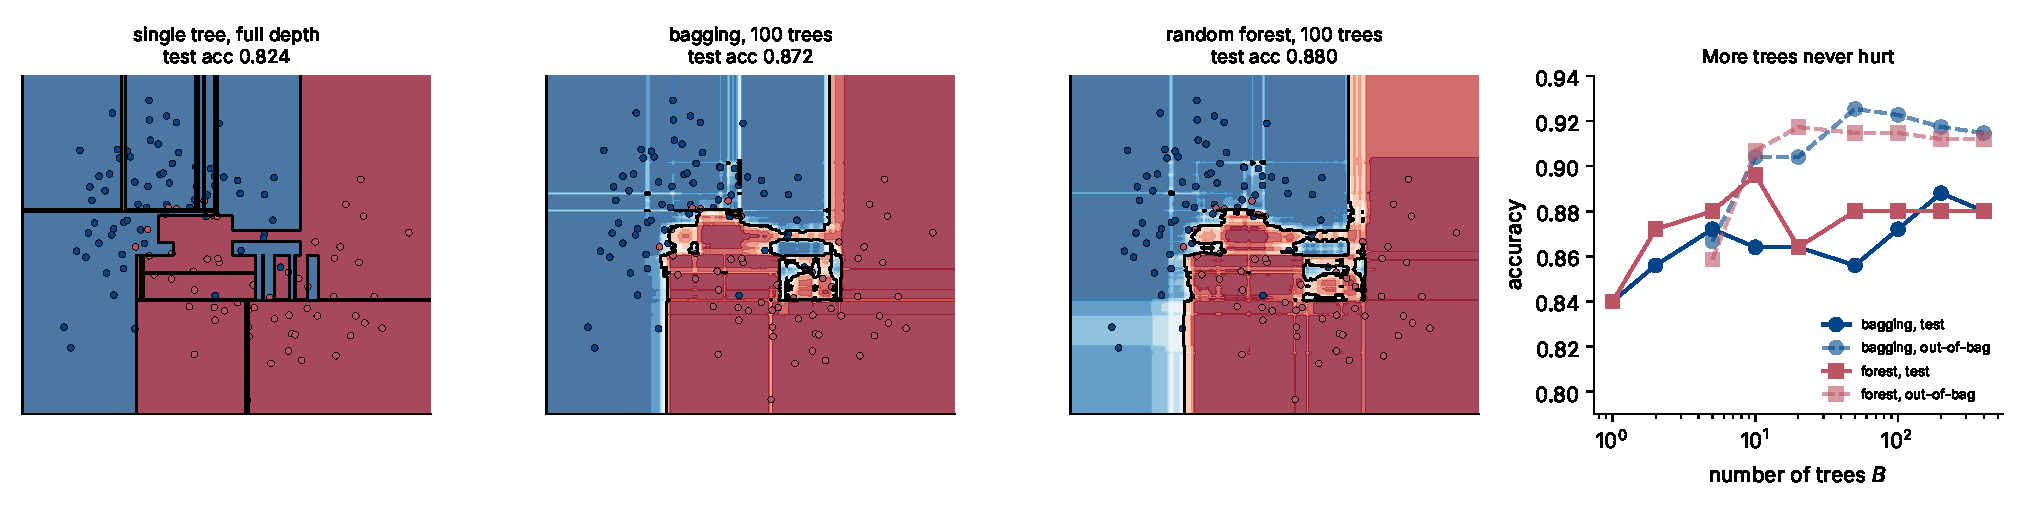
\includegraphics[width=0.98\textwidth]{week46_ensembles.pdf}\\
\small Colour = fraction of trees voting for class 1 (\texttt{predict\_proba});
black line = the majority.  The single tree's islands around individual
points are averaged away; the ensemble boundary is smoother and comes with a
graded confidence.  \textbf{Right}: test and out-of-bag accuracy against
$B$ -- the gain is complete by $B\approx 50$, exactly the saturation of the
second term of Eq.\ (7.16); nothing is lost by going further.
\end{frame}

\begin{frame}[fragile]{Random forests in \texttt{scikit-learn}}
\begin{columns}[T]
\begin{column}{0.54\textwidth}
\begin{lstlisting}[basicstyle=\ttfamily\tiny]
from sklearn.ensemble import (RandomForestClassifier,
                              RandomForestRegressor)

rf = RandomForestClassifier(
        n_estimators=200,       # B: as many as you can afford
        max_features="sqrt",    # m = sqrt(p), Eq. (7.18);
                                # also "log2", an int, a float, None (= bagging)
        max_depth=None,         # grow deep
        min_samples_leaf=1,
        oob_score=True,
        n_jobs=-1,
        random_state=0)
rf.fit(X_train, y_train)
print(rf.oob_score_, rf.score(X_test, y_test))
imp = rf.feature_importances_          # mean Gini decrease
for i in np.argsort(imp)[::-1][:5]:
    print(feature_names[i], round(imp[i], 3))

# regression: max_features defaults to 1.0 (= p, i.e. bagging);
# set max_features=1/3 for the classical rule
rfr = RandomForestRegressor(n_estimators=200, max_features=1/3,
                            oob_score=True).fit(X_train, y_train)
\end{lstlisting}
\end{column}
\begin{column}{0.44\textwidth}
\small
\begin{block}{Two hyperparameters that matter}
\texttt{n\_estimators} ($B$) and \texttt{max\_features} ($m$).  Everything
else is the tree's own knobs, and a forest is remarkably insensitive to them.
\texttt{max\_features=None} turns the forest back into bagging.
\end{block}
\begin{block}{Note the default for regression}
Since version 1.1 \texttt{RandomForestRegressor} uses \emph{all} features
by default -- bagging -- so set \texttt{max\_features} yourself if you want
the decorrelation.
\end{block}
\end{column}
\end{columns}
\end{frame}

\begin{frame}{A real data set: the Wisconsin breast-cancer data}
\small
\begin{columns}[T]
\begin{column}{0.52\textwidth}
569 tumours, 30 features (radius, texture, concavity, \dots), benign or
malignant; 398 training and 171 test points; $B=200$:
\begin{center}
\setlength{\tabcolsep}{3.5pt}
\begin{tabular}{lccc}\toprule
 & train & test & out-of-bag\\\midrule
tree, depth 3 & 0.977 & 0.918 & --\\
tree, full depth (7) & 1.000 & 0.930 & --\\
bagging & 1.000 & 0.942 & 0.955\\
random forest, $m=5$ & 1.000 & 0.953 & 0.957\\
logistic regression, scaled & 0.993 & 0.965 & --\\\bottomrule
\end{tabular}
\end{center}
Mean pairwise correlation between the trees' test predictions:
\textbf{bagging $0.81$, forest $0.78$}.
\end{column}
\begin{column}{0.46\textwidth}
\footnotesize
\begin{block}{Three lessons}
\begin{enumerate}
  \item The ensembles beat the single tree again, by two to three points
        (standard error here $\approx 0.017$).
  \item The forest decorrelates only a little on these data: the 30 features
        are themselves strongly correlated (radius, perimeter, area), so a
        strong one is rarely \emph{all} unavailable.
  \item \textbf{Trees are not always best.}  A scaled logistic regression
        wins on this nearly linearly separable problem.  Forests are the
        safe default on tabular data, not the guaranteed winner.
\end{enumerate}
\end{block}
\end{column}
\end{columns}
\end{frame}

\begin{frame}{Feature importances, and $m$ as a dial for $\rho$}
\centering
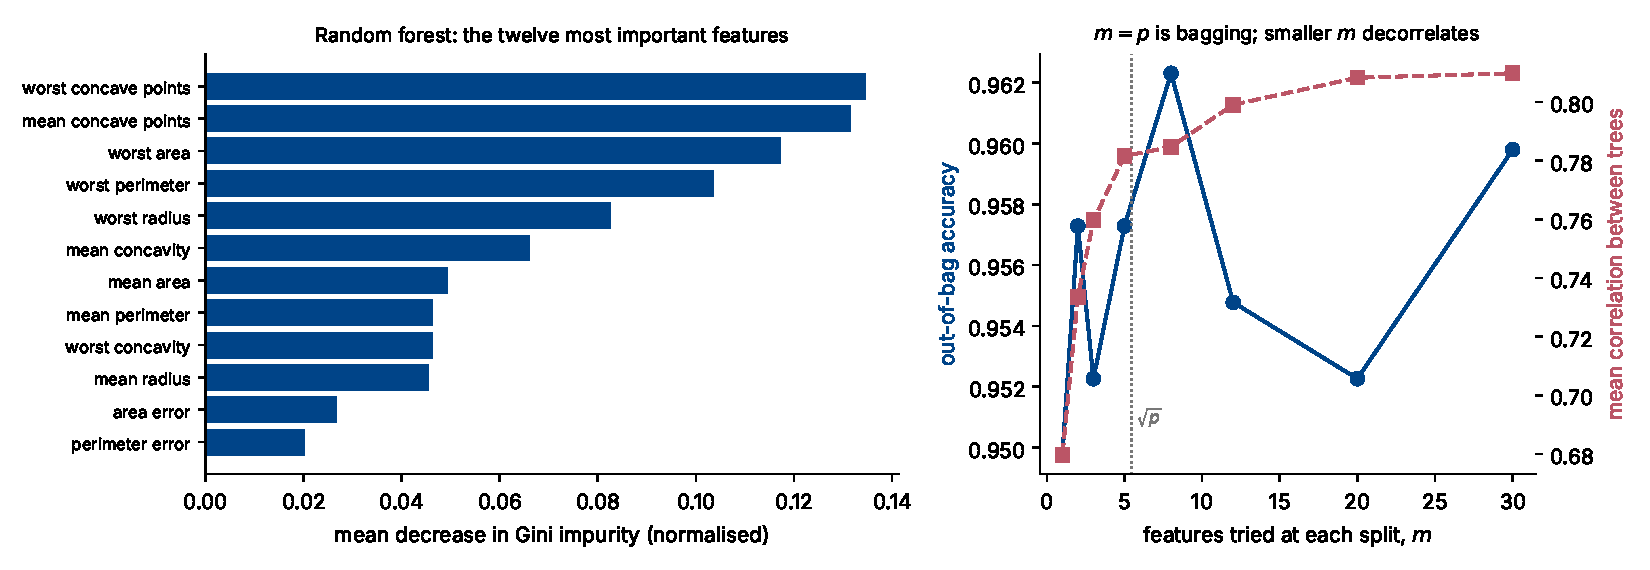
\includegraphics[width=0.98\textwidth]{week46_cancer.pdf}\\
\small
\textbf{Left}: the forest's variable importances -- concave points, area,
perimeter, radius; what replaces the readable tree.  \textbf{Right}: the
mean correlation between trees rises monotonically with $m$, from $0.68$ at
$m=1$ to $0.81$ at $m=p=30$ (bagging), as Eq.\ (7.16) predicts; the
out-of-bag accuracy moves within $\pm 0.005$ -- four tumours -- so on these
data any $m$ from 2 to 30 is as good as any other.  The dial works; here it
has little to turn.
\end{frame}

\begin{insight}[a forest with one feature]
\question{We fit \texttt{RandomForestRegressor} and
\texttt{BaggingRegressor}, 200 deep trees each, to the noisy Runge data of
the regression frame ($p=1$).  Test MSE: single tree at depth 4: $0.0181$,
full depth: $0.0214$; bagging: $0.0173$; forest: $0.0173$; degree-10
polynomial: $0.0133$.  Why are bagging and the forest identical here, why do
they beat the single tree only modestly, and why does the polynomial still win?}
\answer{With $p=1$ there is nothing to subsample: $m=1=p$, and a forest
\emph{is} bagging -- the decorrelation trick needs several features.  The
ensemble removes the variance of the full-depth tree ($0.0214\to0.0173$) but
not its bias: an average of staircases is still a staircase, so the smooth
peak and the flat tails are approximated with the same resolution limit --
and a tree cannot extrapolate past the outermost training points.  A
polynomial is the right inductive bias for one smooth function; trees and
forests earn their keep when there are \emph{many} features, interactions,
mixed types and no good parametric form -- which is most tabular data.}
\end{insight}

\begin{frame}{Random forests as the off-the-shelf method for tabular data}
\begin{columns}[T]
\begin{column}{0.49\textwidth}
\begin{block}{Why people reach for them first}
\begin{itemize}
  \item No feature scaling, insensitive to monotone transformations, mixed
        data types, tolerant of missing values and outliers.
  \item A free error estimate: out-of-bag, Eq.\ (7.17).
  \item Rarely overfit as $B$ grows: more trees only shrink the second term
        of Eq.\ (7.16), never increase the bias.
  \item Essentially two hyperparameters, one of which is ``as many trees as
        you can afford''.
  \item Embarrassingly parallel to train and to predict.
\end{itemize}
\end{block}
\end{column}
\begin{column}{0.49\textwidth}
\begin{block}{Their weaknesses follow from the same structure}
\begin{itemize}
  \item \textbf{No extrapolation}: every prediction is an average of
        observed targets.
  \item Axis-aligned boundaries, staircases for anything diagonal.
  \item Large to store, slow to evaluate compared with a linear model;
        the readable tree is gone.
  \item They attack variance only.  When the single tree is \emph{biased},
        averaging cannot help -- which is where \textbf{boosting} comes in.
\end{itemize}
\end{block}
\end{column}
\end{columns}
\end{frame}

\begin{frame}{Tomorrow, Project 3, and next week}
\begin{columns}[T]
\begin{column}{0.5\textwidth}
\begin{block}{Tomorrow: flipped classroom}
About 20 minutes of questions and answers on today's material -- bring the
things you did not follow (the gain formula, the tie-breaking, the
out-of-bag idea, Eq.\ (7.16)).  Then we go through \textbf{Project 3}
together.
\end{block}
\begin{block}{Project 2}
The deadline is \textbf{today, Monday November 9}.
\end{block}
\end{column}
\begin{column}{0.48\textwidth}
\begin{block}{Reading}
Chapter 7, Sections 7.1--7.10 (7.6 and 7.10 contain the code of today);
Hastie et al.\ 9.2 and 15; the code is in \texttt{week46.ipynb}.
\end{block}
\begin{block}{Next Monday, week 47: boosting}
Many \emph{weak} learners in sequence, each correcting its predecessors --
attacking the bias that averaging leaves alone: AdaBoost and the exponential
loss, gradient boosting as gradient descent in function space, XGBoost, and
boosting any loss with automatic differentiation (Sections 7.11--7.15).
The gated recurrent cells (LSTM, GRU) get their own lecture later.
\end{block}
\end{column}
\end{columns}
\end{frame}

\begin{frame}{Summary of week 46}
\small
\begin{block}{A single tree}
Boxes and constants, grown top-down and greedily.  Splits are scored by an
impurity: MSE for regression, Gini index or entropy for classification --
concave measures, so a pure child is rewarded.  CART minimises the weighted
child impurity $C(k,t)$ of Eq.\ (7.9), i.e.\ maximises the gain (7.10),
over every feature and every midpoint; the ride data and ten points in the
plane showed the arithmetic, and sixty lines of Python reproduce
\texttt{scikit-learn}.  A full-depth tree has zero training error and large
variance.
\end{block}
\begin{block}{Many trees}
$\var(\bar f)=\rho\sigma^2+\tfrac{1-\rho}{B}\sigma^2$ (7.16).  Bagging:
bootstrap samples, deep trees, average or vote, out-of-bag error for free
(7.17); it shrinks the second term.  Random forests: $m\approx\sqrt p$
random features per split (7.18); it lowers $\rho$, hence the floor.
Both beat a single tree by a wide margin and are hard to overfit with $B$;
neither can extrapolate or reduce bias.
\end{block}
\begin{block}{Next}
Boosting: the route that attacks the bias.
\end{block}
\end{frame}

\end{document}
